% ======================================================================
% CampusTrack - User Manual
% Compile with pdflatex (works on Overleaf, MiKTeX, TeX Live)
% ======================================================================
\documentclass[11pt,a4paper]{report}

\usepackage[margin=2.4cm]{geometry}
\usepackage[T1]{fontenc}
\usepackage{lmodern}
\usepackage{graphicx}
\usepackage{xcolor}
\usepackage{amssymb}
\usepackage{tikz}
\usetikzlibrary{positioning,arrows.meta}
\usepackage{enumitem}
\usepackage{booktabs}
\usepackage{float}

\definecolor{campusblue}{RGB}{26,86,168}
\definecolor{lightbg}{RGB}{244,246,250}
\definecolor{okgreen}{RGB}{10,125,56}
\definecolor{warnorange}{RGB}{220,120,20}

\usepackage[colorlinks=true,linkcolor=campusblue,urlcolor=campusblue]{hyperref}

\graphicspath{{images/}}

% ---------- simple "tip" and "note" boxes -----------------------------
\newcommand{\tipbox}[1]{%
  \begin{center}
  \fcolorbox{campusblue}{lightbg}{\parbox{0.92\textwidth}{\small \textbf{Tip:} #1}}
  \end{center}}
\newcommand{\notebox}[1]{%
  \begin{center}
  \fcolorbox{warnorange}{lightbg}{\parbox{0.92\textwidth}{\small \textbf{Note:} #1}}
  \end{center}}

% ---------- phone mock-up helpers (TikZ) ------------------------------
% \appcard{y}{right symbol}{bold line}{grey line}
\newcommand{\appcard}[4]{%
  \draw[rounded corners=3pt, fill=white, draw=black!15] (0.25,#1) rectangle (4.95,#1+1.05);
  \node[anchor=west] at (0.45,#1+0.70) {\footnotesize\textbf{#3}};
  \node[anchor=west, text=black!55] at (0.45,#1+0.32) {\scriptsize #4};
  \node[anchor=east, text=campusblue] at (4.80,#1+0.52) {\small #2};}

% \phoneframe{app bar title}   ... draw inside a tikzpicture
\newcommand{\phoneframe}[1]{%
  \draw[rounded corners=14pt, fill=lightbg, draw=black!60, line width=1.2pt]
        (0,0) rectangle (5.2,9.8);
  \fill[campusblue] (0.06,8.9) rectangle (5.14,9.55);
  \node[text=white, anchor=west] at (0.35,9.22) {\small\textbf{#1}};}

% bottom navigation bar: draw the bar, then place items with \navitem
\newcommand{\navbar}{%
  \draw[fill=white, draw=black!20] (0.06,0.08) rectangle (5.14,0.75);}
% \navitem{x}{label}{color}
\newcommand{\navitem}[3]{\node[text=#3] at (#1,0.42) {\tiny #2};}

% ======================================================================
\begin{document}

% ---------------- title page ----------------
\begin{titlepage}
\centering
\vspace*{2cm}
{\Huge\bfseries\color{campusblue} CampusTrack\par}
\vspace{0.4cm}
{\LARGE RFID School \& College Management System\par}
\vspace{1.2cm}
{\Large\bfseries User Manual\par}
\vspace{0.4cm}
{\large For Parents, Students, Teachers and Administrators\par}
\vspace{2cm}
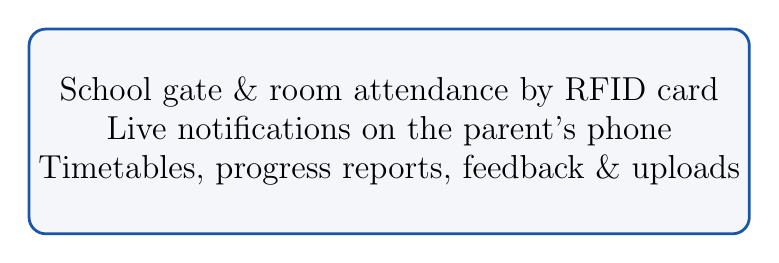
\begin{tikzpicture}
  \node[draw=campusblue, rounded corners=6pt, line width=1pt,
        minimum width=9cm, minimum height=2.6cm, fill=lightbg, align=center]
    {\large School gate \& room attendance by RFID card\\[2pt]
     \large Live notifications on the parent's phone\\[2pt]
     \large Timetables, progress reports, feedback \& uploads};
\end{tikzpicture}
\vfill
{\large Version 1.0 \par}
{\large August 2026 \par}
\end{titlepage}

\tableofcontents

\chapter{Welcome to CampusTrack}

\section{What is CampusTrack?}

CampusTrack is a complete software system for schools and colleges. It
connects four groups of people:

\begin{itemize}[itemsep=2pt]
  \item \textbf{Parents} -- see, on their own phone, when their child
        arrives at school and leaves school, which rooms and classes the
        child attended, the full semester timetable, and progress
        reports written by teachers. Parents can also send feedback to
        the school and receive replies.
  \item \textbf{Students} -- see their timetable, download assignments
        and notes by scanning a QR code, and upload their projects,
        activities and theses from their phone.
  \item \textbf{Teachers} -- use a website to write progress updates
        about students, publish assignments and notes, answer parent
        feedback, and review student uploads.
  \item \textbf{Administrators} -- manage everything: classes, sections,
        rooms, RFID readers, timetables and user accounts. Classes and
        sections are \emph{modular}: the admin can add or remove them at
        any time.
\end{itemize}

\section{How does the attendance work? (in plain words)}

Every student carries a normal-looking \textbf{ID card}. Inside the card
there is a tiny \textbf{RFID chip} -- like the chip in a contactless bus
card. The student does not need to touch anything or stand in a queue.

At the \textbf{school gate} and in \textbf{every room} (classrooms,
laboratories, library, discussion rooms, auditorium) there are small
\textbf{antennas} fixed above the door. When a student simply walks
through, the antennas notice the card -- automatically, from a distance.

\subsection{How the system knows IN from OUT}

The trick is the \emph{order} in which the antennas see the card:

\begin{itemize}
  \item Walking \textbf{in}, the card passes antenna 1 first, then 2,
        then 3 (at the gate).
  \item Walking \textbf{out}, the same antennas see the card in the
        reverse order: 3, then 2, then 1.
\end{itemize}

\begin{figure}[H]
\centering
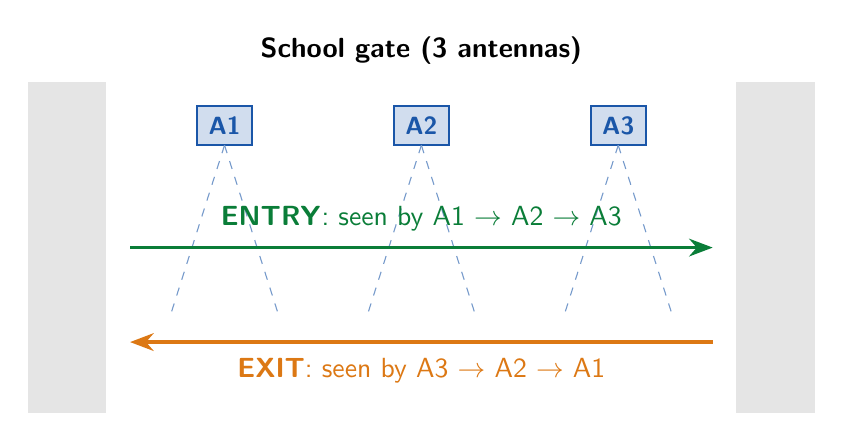
\begin{tikzpicture}[font=\sffamily, >={Stealth[length=3mm]}]
  % gate structure
  \fill[black!10] (0,0) rectangle (1.0,4.2);
  \fill[black!10] (9.0,0) rectangle (10.0,4.2);
  \node at (5,4.6) {\textbf{School gate (3 antennas)}};
  % antennas
  \foreach \x/\n in {2.5/1, 5.0/2, 7.5/3}{
     \draw[fill=campusblue!20, draw=campusblue, thick] (\x-0.35,3.4) rectangle (\x+0.35,3.9);
     \node[text=campusblue] at (\x,3.65) {\small\textbf{A\n}};
     \draw[campusblue!60, dashed] (\x,3.4) -- (\x-0.7,1.2);
     \draw[campusblue!60, dashed] (\x,3.4) -- (\x+0.7,1.2);
  }
  % entry arrow
  \draw[->, very thick, okgreen] (1.3,2.1) -- (8.7,2.1)
     node[midway, above=2pt, text=okgreen] {\textbf{ENTRY}: seen by A1 $\rightarrow$ A2 $\rightarrow$ A3};
  % exit arrow
  \draw[->, very thick, warnorange] (8.7,0.9) -- (1.3,0.9)
     node[midway, below=2pt, text=warnorange] {\textbf{EXIT}: seen by A3 $\rightarrow$ A2 $\rightarrow$ A1};
\end{tikzpicture}
\caption{The gate has three antennas. The order in which they detect the
ID card tells the system whether the student walked in or out.}
\end{figure}

Rooms work exactly the same way, only with \textbf{two} antennas:
antenna 1 then antenna 2 means the student \textbf{entered} the room;
antenna 2 then antenna 1 means the student \textbf{left} the room.

\begin{figure}[H]
\centering
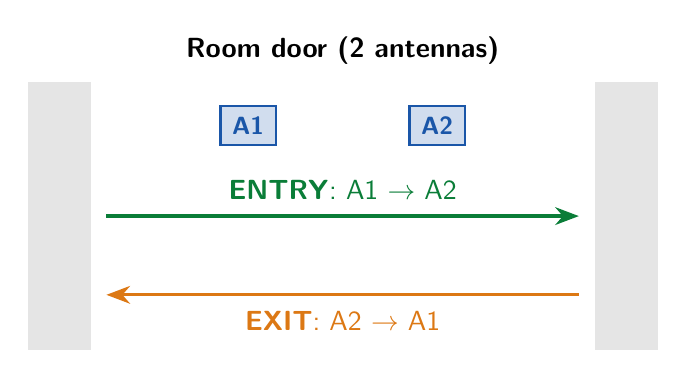
\begin{tikzpicture}[font=\sffamily, >={Stealth[length=3mm]}]
  \fill[black!10] (0,0) rectangle (0.8,3.4);
  \fill[black!10] (7.2,0) rectangle (8.0,3.4);
  \node at (4,3.8) {\textbf{Room door (2 antennas)}};
  \foreach \x/\n in {2.8/1, 5.2/2}{
     \draw[fill=campusblue!20, draw=campusblue, thick] (\x-0.35,2.6) rectangle (\x+0.35,3.1);
     \node[text=campusblue] at (\x,2.85) {\small\textbf{A\n}};
  }
  \draw[->, very thick, okgreen] (1.0,1.7) -- (7.0,1.7)
     node[midway, above=2pt, text=okgreen] {\textbf{ENTRY}: A1 $\rightarrow$ A2};
  \draw[->, very thick, warnorange] (7.0,0.7) -- (1.0,0.7)
     node[midway, below=2pt, text=warnorange] {\textbf{EXIT}: A2 $\rightarrow$ A1};
\end{tikzpicture}
\caption{Every classroom, laboratory, library, discussion room and
auditorium door has two antennas using the same idea.}
\end{figure}

\section{What happens after a student is detected?}

\begin{enumerate}[itemsep=2pt]
  \item The moment a student walks through the \textbf{gate}, the
        parent's phone receives a notification: \emph{``Ali Khan entered
        school at 07:58''} (and the same when the student leaves).
  \item Every room the student enters during the day is silently
        recorded.
  \item Every evening (at 6:00 pm by default) the parent receives a
        \textbf{daily summary}: arrival time, departure time, rooms and
        classes attended, and any teacher remarks of the day.
  \item Every Friday the parent receives a \textbf{weekly summary} of
        the whole week.
\end{enumerate}

\section{The parts of the system}

\begin{figure}[H]
\centering
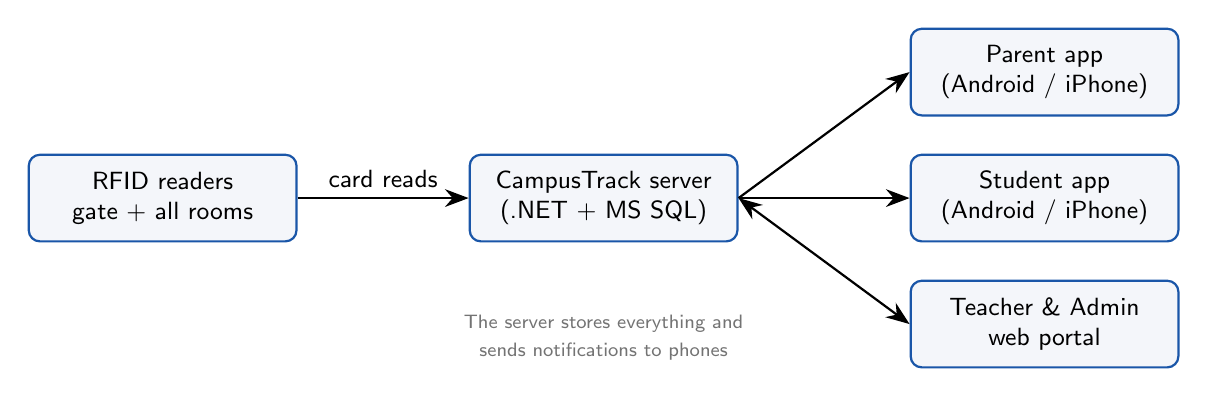
\begin{tikzpicture}[font=\sffamily\small, >={Stealth[length=3mm]},
    box/.style={draw=campusblue, fill=lightbg, rounded corners=4pt,
                minimum width=3.4cm, minimum height=1.1cm, align=center, thick}]
  \node[box] (readers) at (0,0)   {RFID readers\\ gate + all rooms};
  \node[box] (server)  at (5.6,0) {CampusTrack server\\ (.NET + MS SQL)};
  \node[box] (parent)  at (11.2,1.6)  {Parent app\\ (Android / iPhone)};
  \node[box] (student) at (11.2,0)    {Student app\\ (Android / iPhone)};
  \node[box] (portal)  at (11.2,-1.6) {Teacher \& Admin\\ web portal};
  \draw[->, thick] (readers) -- node[above]{card reads} (server);
  \draw[->, thick] (server.east) -- (parent.west);
  \draw[->, thick] (server.east) -- (student.west);
  \draw[<->, thick] (server.east) -- (portal.west);
  \node[text=black!55] at (5.6,-1.6) {\scriptsize The server stores everything and};
  \node[text=black!55] at (5.6,-1.95) {\scriptsize sends notifications to phones};
\end{tikzpicture}
\caption{How the pieces connect. The readers watch the doors, the server
keeps the records, and each person sees their own portal.}
\end{figure}

\notebox{Nobody needs to understand the technology to use CampusTrack.
Parents and students only install one app and log in. Teachers and
admins only open a website.}

\chapter{Getting started}

\section{Who uses what}

\begin{table}[H]
\centering
\begin{tabular}{lll}
\toprule
\textbf{You are a\ldots} & \textbf{You use\ldots} & \textbf{Where} \\
\midrule
Parent  & CampusTrack mobile app & your own phone \\
Student & CampusTrack mobile app & your own phone \\
Teacher & Teacher \& Admin web portal & any browser \\
Admin   & Teacher \& Admin web portal & any browser \\
\bottomrule
\end{tabular}
\caption{One mobile app serves both parents and students -- the app
shows the right portal automatically after login.}
\end{table}

\section{Your username and password}

You do \textbf{not} register yourself. The school office (the
administrator) creates an account for every parent, student and teacher
and hands over the username and password. If you forget your password,
contact the school office -- they can set a new one.

\section{Installing the mobile app (parents and students)}

\begin{enumerate}[itemsep=2pt]
  \item Install \textbf{CampusTrack} from the Google Play Store
        (Android) or the App Store (iPhone) -- or from the link the
        school gives you.
  \item Open the app. You will see the sign-in screen.
  \item Type the username and password the school gave you and tap
        \textbf{Sign in}.
  \item When the phone asks \emph{``Allow notifications?''} tap
        \textbf{Allow} -- otherwise you will not receive gate alerts and
        daily summaries.
\end{enumerate}

\begin{figure}[H]
\centering
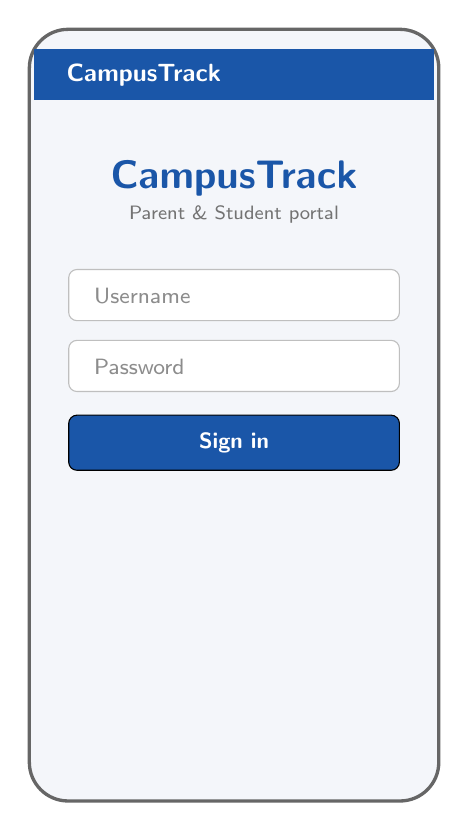
\begin{tikzpicture}[font=\sffamily]
  \phoneframe{CampusTrack}
  \node[text=campusblue] at (2.6,7.9) {\Large\textbf{CampusTrack}};
  \node[text=black!55] at (2.6,7.45) {\scriptsize Parent \& Student portal};
  \draw[rounded corners=3pt, fill=white, draw=black!25] (0.5,6.1) rectangle (4.7,6.75);
  \node[anchor=west, text=black!45] at (0.7,6.42) {\footnotesize Username};
  \draw[rounded corners=3pt, fill=white, draw=black!25] (0.5,5.2) rectangle (4.7,5.85);
  \node[anchor=west, text=black!45] at (0.7,5.52) {\footnotesize Password};
  \draw[rounded corners=3pt, fill=campusblue] (0.5,4.2) rectangle (4.7,4.9);
  \node[text=white] at (2.6,4.55) {\footnotesize\textbf{Sign in}};
\end{tikzpicture}
\caption{The sign-in screen of the mobile app (illustration).}
\end{figure}

\section{Opening the web portal (teachers and admins)}

\begin{enumerate}[itemsep=2pt]
  \item Open any browser (Chrome, Edge, Firefox).
  \item Go to the school's CampusTrack address, for example\\
        \texttt{https://campustrack.yourschool.edu}
  \item Sign in with your teacher or admin username.
\end{enumerate}

\begin{figure}[H]
\centering
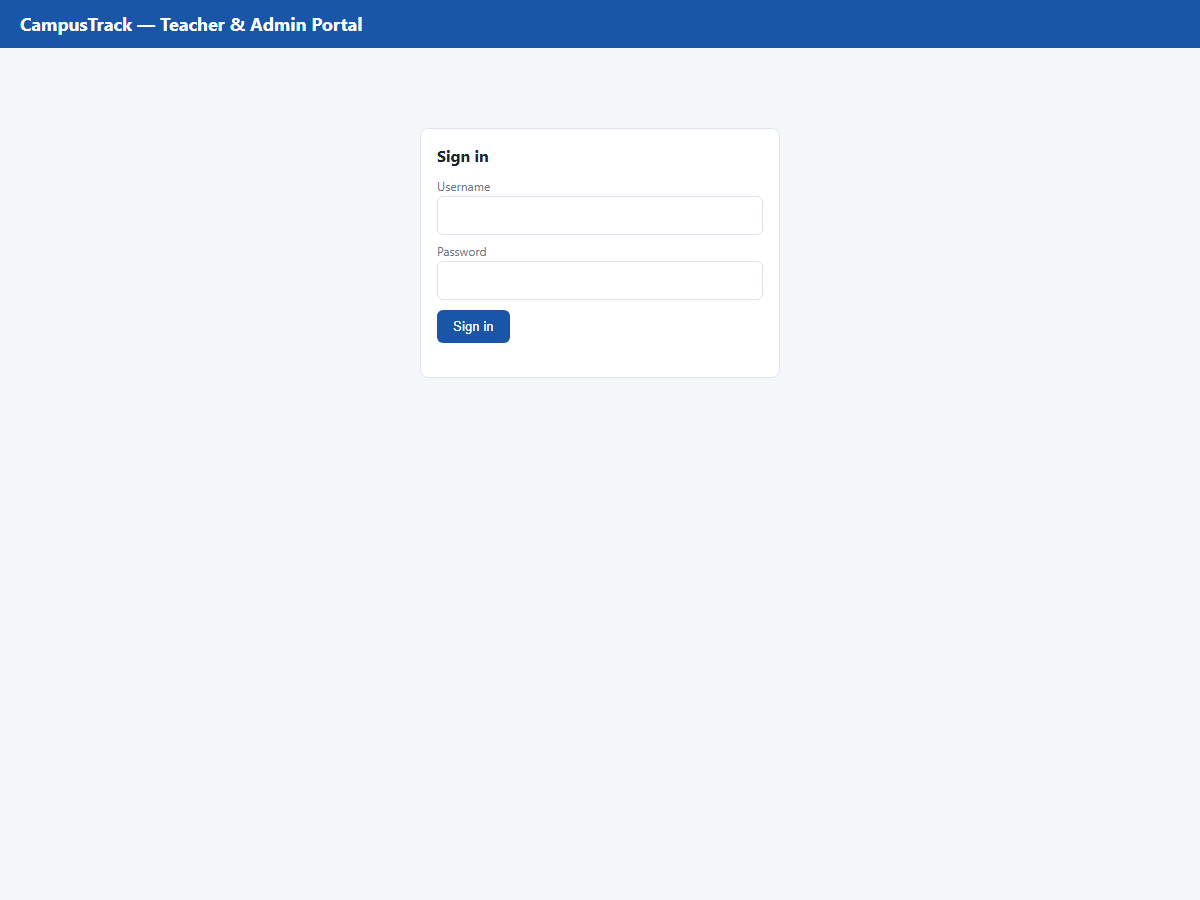
\includegraphics[width=0.8\textwidth]{portal-login}
\caption{The web portal sign-in page (actual screenshot).}
\end{figure}

\notebox{The web portal is only for teachers and administrators. If a
parent or student signs in there, the portal politely refuses and points
them to the mobile app.}

\chapter{Parent Portal (mobile app)}

After signing in, a parent sees five buttons at the bottom of the
screen:

\begin{center}
\textbf{Attendance} \quad \textbf{Schedule} \quad \textbf{Activity}
\quad \textbf{Feedback} \quad \textbf{Alerts}
\end{center}

If you have more than one child in the school, a small selector at the
top of the screen lets you switch between children -- everything on the
screen then shows that child's information.

% ----------------------------------------------------------------------
\section{Attendance -- was my child at school?}

The \textbf{Attendance} tab has two views, switchable at the top:

\subsection{Daily view}
One line per day: a green tick if the child was present, the
\textbf{arrival time} at the gate and the \textbf{departure time}.

\subsection{Movements view}
The full trail of the day, recorded automatically by the room antennas:
entered Room 101 at 08:02, left at 08:59, entered the Library at 10:15,
and so on. Nothing needs to be typed by anyone -- walking through a door
is enough.

\begin{figure}[H]
\centering
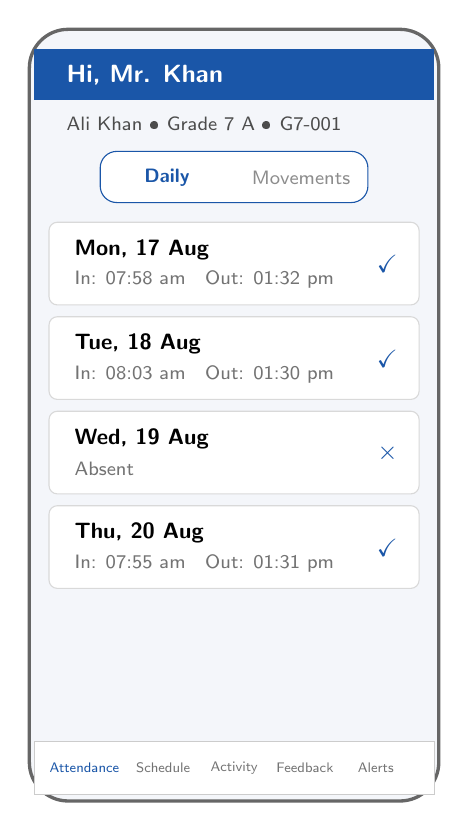
\begin{tikzpicture}[font=\sffamily]
  \phoneframe{Hi, Mr. Khan}
  \node[anchor=west, text=black!70] at (0.35,8.60) {\scriptsize Ali Khan \textbullet{}  Grade 7 A \textbullet{}  G7-001};
  \draw[rounded corners=6pt, fill=white, draw=campusblue] (0.9,7.6) rectangle (4.3,8.25);
  \node[text=campusblue] at (1.75,7.92) {\scriptsize\textbf{Daily}};
  \node[text=black!45] at (3.45,7.92) {\scriptsize Movements};
  \appcard{6.3}{\checkmark}{Mon, 17 Aug}{In: 07:58 am \; Out: 01:32 pm}
  \appcard{5.1}{\checkmark}{Tue, 18 Aug}{In: 08:03 am \; Out: 01:30 pm}
  \appcard{3.9}{$\times$}{Wed, 19 Aug}{Absent}
  \appcard{2.7}{\checkmark}{Thu, 20 Aug}{In: 07:55 am \; Out: 01:31 pm}
  \navbar
  \navitem{0.70}{Attendance}{campusblue}
  \navitem{1.70}{Schedule}{black!55}
  \navitem{2.60}{Activity}{black!55}
  \navitem{3.50}{Feedback}{black!55}
  \navitem{4.40}{Alerts}{black!55}
\end{tikzpicture}
\hspace{0.8cm}
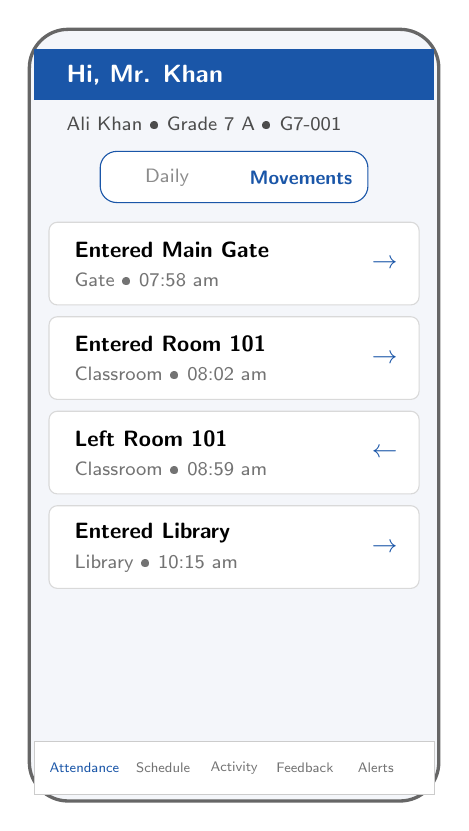
\begin{tikzpicture}[font=\sffamily]
  \phoneframe{Hi, Mr. Khan}
  \node[anchor=west, text=black!70] at (0.35,8.60) {\scriptsize Ali Khan \textbullet{}  Grade 7 A \textbullet{}  G7-001};
  \draw[rounded corners=6pt, fill=white, draw=campusblue] (0.9,7.6) rectangle (4.3,8.25);
  \node[text=black!45] at (1.75,7.92) {\scriptsize Daily};
  \node[text=campusblue] at (3.45,7.92) {\scriptsize\textbf{Movements}};
  \appcard{6.3}{$\rightarrow$}{Entered Main Gate}{Gate \textbullet{}  07:58 am}
  \appcard{5.1}{$\rightarrow$}{Entered Room 101}{Classroom \textbullet{}  08:02 am}
  \appcard{3.9}{$\leftarrow$}{Left Room 101}{Classroom \textbullet{}  08:59 am}
  \appcard{2.7}{$\rightarrow$}{Entered Library}{Library \textbullet{}  10:15 am}
  \navbar
  \navitem{0.70}{Attendance}{campusblue}
  \navitem{1.70}{Schedule}{black!55}
  \navitem{2.60}{Activity}{black!55}
  \navitem{3.50}{Feedback}{black!55}
  \navitem{4.40}{Alerts}{black!55}
\end{tikzpicture}
\caption{Attendance tab: the Daily view (left) and the room-by-room
Movements view (right). Illustrations of the app screens.}
\end{figure}

\tipbox{Pull the list downwards with your finger to refresh it.}

% ----------------------------------------------------------------------
\section{Schedule -- the full semester timetable}

Tap \textbf{Schedule} to see your child's timetable for the whole
semester, day by day: subject, time, teacher and room. Whenever the
school updates the timetable, the app always shows the latest version --
no paper needed.

\begin{figure}[H]
\centering
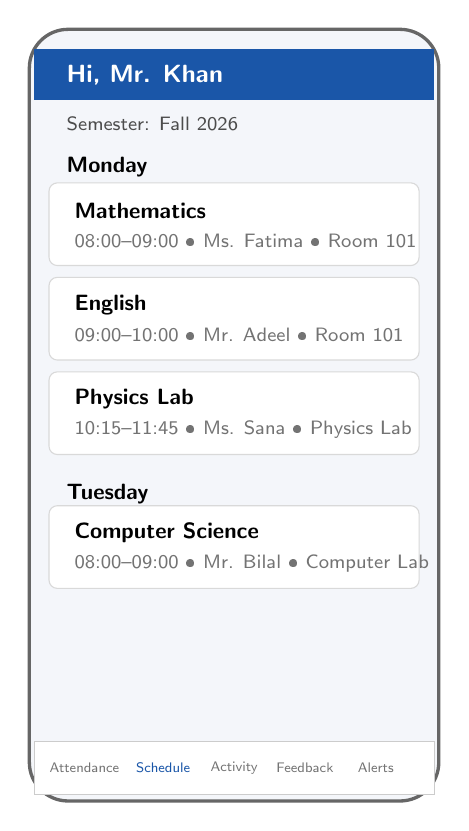
\begin{tikzpicture}[font=\sffamily]
  \phoneframe{Hi, Mr. Khan}
  \node[anchor=west, text=black!70] at (0.35,8.60) {\scriptsize Semester: Fall 2026};
  \node[anchor=west] at (0.35,8.05) {\footnotesize\textbf{Monday}};
  \appcard{6.8}{}{Mathematics}{08:00--09:00 \textbullet{}  Ms. Fatima \textbullet{}  Room 101}
  \appcard{5.6}{}{English}{09:00--10:00 \textbullet{}  Mr. Adeel \textbullet{}  Room 101}
  \appcard{4.4}{}{Physics Lab}{10:15--11:45 \textbullet{}  Ms. Sana \textbullet{}  Physics Lab}
  \node[anchor=west] at (0.35,3.9) {\footnotesize\textbf{Tuesday}};
  \appcard{2.7}{}{Computer Science}{08:00--09:00 \textbullet{}  Mr. Bilal \textbullet{}  Computer Lab}
  \navbar
  \navitem{0.70}{Attendance}{black!55}
  \navitem{1.70}{Schedule}{campusblue}
  \navitem{2.60}{Activity}{black!55}
  \navitem{3.50}{Feedback}{black!55}
  \navitem{4.40}{Alerts}{black!55}
\end{tikzpicture}
\caption{Schedule tab: the whole semester, grouped by day
(illustration).}
\end{figure}

% ----------------------------------------------------------------------
\section{Activity -- what teachers say about my child}

Tap \textbf{Activity} to read every report a teacher has written about
your child: test results, homework status, behaviour notes, sports
achievements. Each report shows the category, the date, the teacher's
name, the remarks and (when given) a grade.

You do not have to keep checking: whenever a teacher writes a new
report, your phone receives a notification immediately.

\begin{figure}[H]
\centering
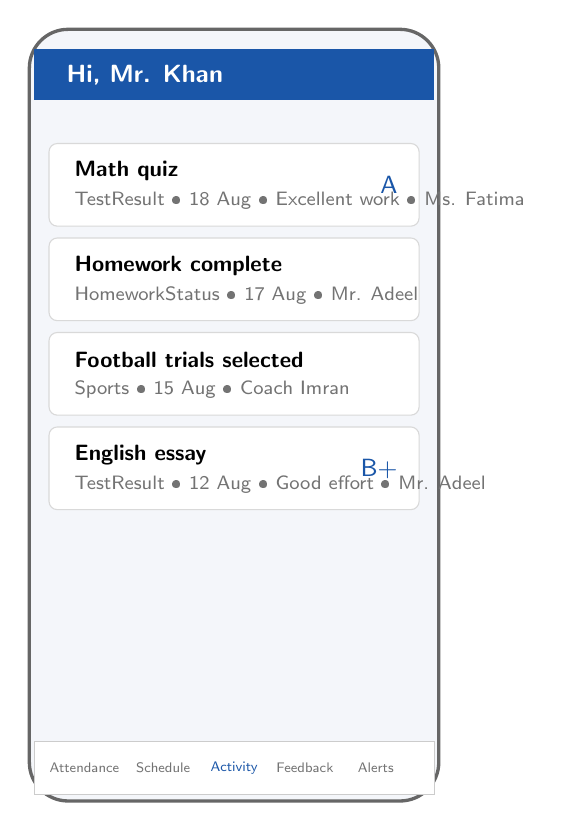
\begin{tikzpicture}[font=\sffamily]
  \phoneframe{Hi, Mr. Khan}
  \appcard{7.3}{A}{Math quiz}{TestResult \textbullet{}  18 Aug \textbullet{}  Excellent work \textbullet{}  Ms. Fatima}
  \appcard{6.1}{}{Homework complete}{HomeworkStatus \textbullet{}  17 Aug \textbullet{}  Mr. Adeel}
  \appcard{4.9}{}{Football trials selected}{Sports \textbullet{}  15 Aug \textbullet{}  Coach Imran}
  \appcard{3.7}{B+}{English essay}{TestResult \textbullet{}  12 Aug \textbullet{}  Good effort \textbullet{}  Mr. Adeel}
  \navbar
  \navitem{0.70}{Attendance}{black!55}
  \navitem{1.70}{Schedule}{black!55}
  \navitem{2.60}{Activity}{campusblue}
  \navitem{3.50}{Feedback}{black!55}
  \navitem{4.40}{Alerts}{black!55}
\end{tikzpicture}
\caption{Activity tab: all teacher reports in one place
(illustration).}
\end{figure}

% ----------------------------------------------------------------------
\section{Feedback -- talk to the school}

Tap \textbf{Feedback} to send a message to the school in one of the
fixed columns (categories):

\begin{center}
Teaching \; \textbullet{}  \; Homework \; \textbullet{}  \; Facilities \; \textbullet{}  \; Transport \; \textbullet{}  \;
Discipline \; \textbullet{}  \; Suggestion \; \textbullet{}  \; Complaint
\end{center}

\begin{enumerate}[itemsep=2pt]
  \item Choose which child the feedback is about (if you have several).
  \item Choose the category from the list.
  \item Type your message and tap \textbf{Submit}.
\end{enumerate}

Below the form you can see all your earlier messages, their status
(Open / Replied / Closed) and the school's written reply. When the
school replies, you also get a phone notification.

\begin{figure}[H]
\centering
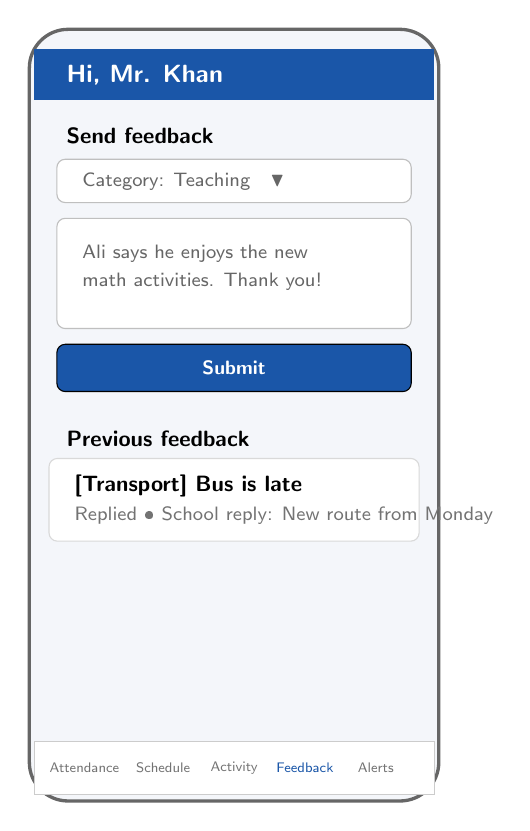
\begin{tikzpicture}[font=\sffamily]
  \phoneframe{Hi, Mr. Khan}
  \node[anchor=west] at (0.35,8.45) {\footnotesize\textbf{Send feedback}};
  \draw[rounded corners=3pt, fill=white, draw=black!25] (0.35,7.6) rectangle (4.85,8.15);
  \node[anchor=west, text=black!60] at (0.55,7.87) {\scriptsize Category: Teaching \; $\blacktriangledown$};
  \draw[rounded corners=3pt, fill=white, draw=black!25] (0.35,6.0) rectangle (4.85,7.4);
  \node[anchor=west, text=black!60] at (0.55,6.95) {\scriptsize Ali says he enjoys the new};
  \node[anchor=west, text=black!60] at (0.55,6.60) {\scriptsize math activities. Thank you!};
  \draw[rounded corners=3pt, fill=campusblue] (0.35,5.2) rectangle (4.85,5.8);
  \node[text=white] at (2.6,5.5) {\scriptsize\textbf{Submit}};
  \node[anchor=west] at (0.35,4.6) {\footnotesize\textbf{Previous feedback}};
  \appcard{3.3}{}{[Transport] Bus is late}{Replied \textbullet{}  School reply: New route from Monday}
  \navbar
  \navitem{0.70}{Attendance}{black!55}
  \navitem{1.70}{Schedule}{black!55}
  \navitem{2.60}{Activity}{black!55}
  \navitem{3.50}{Feedback}{campusblue}
  \navitem{4.40}{Alerts}{black!55}
\end{tikzpicture}
\caption{Feedback tab: fixed categories, your message, and the school's
replies below (illustration).}
\end{figure}

% ----------------------------------------------------------------------
\section{Alerts -- every notification in one list}

Tap \textbf{Alerts} to see everything the school has sent you:

\begin{itemize}[itemsep=2pt]
  \item \textbf{Gate alerts} -- ``Ali Khan entered school at 07:58''
        the moment it happens;
  \item \textbf{Daily summary} -- every evening: arrival, departure,
        rooms attended, teacher updates of the day;
  \item \textbf{Weekly summary} -- every Friday, the whole week at a
        glance;
  \item \textbf{Activity alerts} -- a teacher wrote a new report;
  \item \textbf{Feedback replies} -- the school answered your message.
\end{itemize}

Unread notifications are shown in bold; tap one to mark it as read.

\begin{figure}[H]
\centering
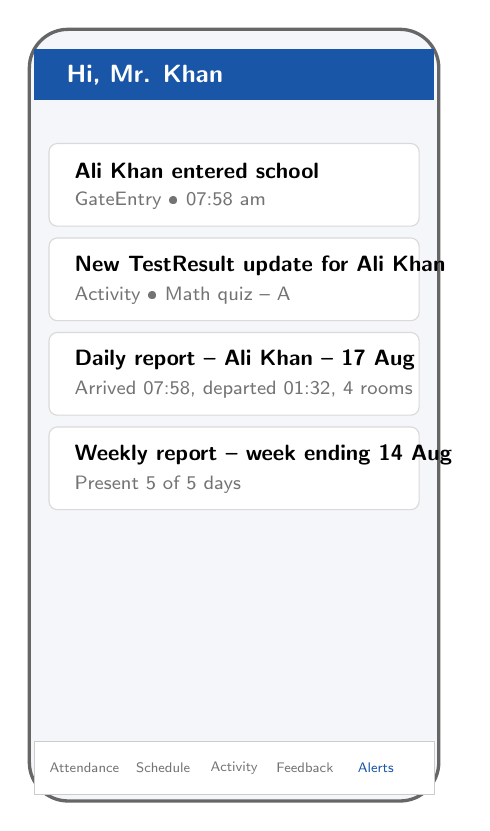
\begin{tikzpicture}[font=\sffamily]
  \phoneframe{Hi, Mr. Khan}
  \appcard{7.3}{}{Ali Khan entered school}{GateEntry \textbullet{}  07:58 am}
  \appcard{6.1}{}{New TestResult update for Ali Khan}{Activity \textbullet{}  Math quiz -- A}
  \appcard{4.9}{}{Daily report -- Ali Khan -- 17 Aug}{Arrived 07:58, departed 01:32, 4 rooms}
  \appcard{3.7}{}{Weekly report -- week ending 14 Aug}{Present 5 of 5 days}
  \navbar
  \navitem{0.70}{Attendance}{black!55}
  \navitem{1.70}{Schedule}{black!55}
  \navitem{2.60}{Activity}{black!55}
  \navitem{3.50}{Feedback}{black!55}
  \navitem{4.40}{Alerts}{campusblue}
\end{tikzpicture}
\caption{Alerts tab: gate events, daily and weekly summaries, teacher
updates and replies (illustration).}
\end{figure}

\chapter{Student Portal (mobile app)}

Students sign in to the \emph{same} app as parents, with their own
username. The app recognises the student account and shows four buttons
at the bottom:

\begin{center}
\textbf{Schedule} \quad \textbf{Assignments} \quad \textbf{My work}
\quad \textbf{Alerts}
\end{center}

% ----------------------------------------------------------------------
\section{Schedule -- my timetable}

Exactly like the parent view: the full semester timetable, day by day,
with subject, time, teacher and room. Check it every morning to know
where to go.

% ----------------------------------------------------------------------
\section{Assignments -- download assignments and notes}

The \textbf{Assignments} tab lists every assignment and every notes
file your teachers have published for your section, newest first. Each
row shows the title, the teacher, and the due date (for assignments).

There are \textbf{two ways to get the file}:

\subsection{Way 1: tap the download button}
Simply tap the download icon on the row -- the file opens on your
phone.

\subsection{Way 2: scan the QR code (even faster in class)}
When a teacher hands out an assignment, the printout (or the projector
screen) carries a small square \textbf{QR code}.

\begin{enumerate}[itemsep=2pt]
  \item Tap the round \textbf{Scan QR} button at the bottom right.
  \item Point the camera at the QR code.
  \item The file downloads immediately -- nothing to type.
\end{enumerate}

\begin{figure}[H]
\centering
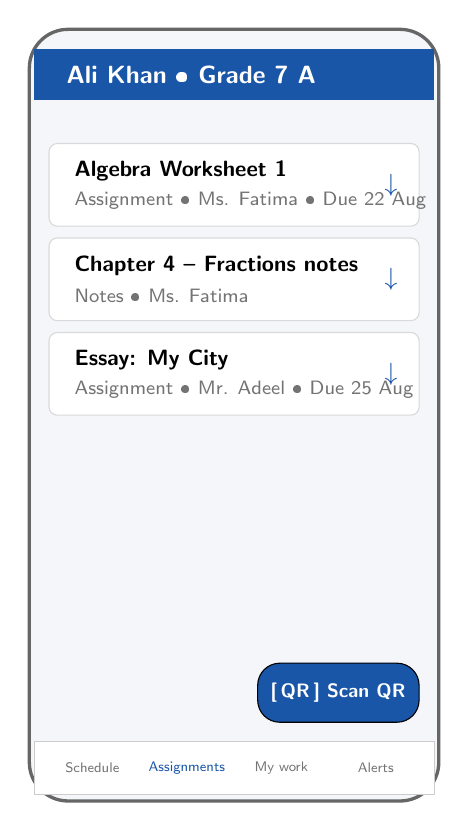
\begin{tikzpicture}[font=\sffamily]
  \phoneframe{Ali Khan \textbullet{}  Grade 7 A}
  \appcard{7.3}{$\downarrow$}{Algebra Worksheet 1}{Assignment \textbullet{}  Ms. Fatima \textbullet{}  Due 22 Aug}
  \appcard{6.1}{$\downarrow$}{Chapter 4 -- Fractions notes}{Notes \textbullet{}  Ms. Fatima}
  \appcard{4.9}{$\downarrow$}{Essay: My City}{Assignment \textbullet{}  Mr. Adeel \textbullet{}  Due 25 Aug}
  \draw[rounded corners=8pt, fill=campusblue] (2.9,1.0) rectangle (4.95,1.75);
  \node[text=white] at (3.92,1.37) {\scriptsize\textbf{[\,QR\,] Scan QR}};
  \navbar
  \navitem{0.80}{Schedule}{black!55}
  \navitem{2.00}{Assignments}{campusblue}
  \navitem{3.20}{My work}{black!55}
  \navitem{4.40}{Alerts}{black!55}
\end{tikzpicture}
\hspace{0.8cm}
\begin{minipage}[b]{4.5cm}
\centering

\includegraphics[width=3.2cm]{qr-sample}\\[4pt]
\scriptsize A real CampusTrack assignment QR code generated by the
system. Scanning it with the app downloads the file
``Algebra Worksheet 1''.
\vspace{2.2cm}
\end{minipage}
\caption{Left: the Assignments tab with the Scan QR button
(illustration). Right: an actual QR code produced by the software.}
\end{figure}

\notebox{The app only accepts CampusTrack QR codes. If you scan
something else -- a shop QR, a random poster -- the app politely says it
is not an assignment code.}

% ----------------------------------------------------------------------
\section{My work -- upload projects, activities and theses}

The \textbf{My work} tab is where you hand in your work from your
phone:

\begin{enumerate}[itemsep=2pt]
  \item Tap the \textbf{+} button.
  \item Choose the type: \textbf{Project}, \textbf{Activity} or
        \textbf{Thesis}.
  \item Type a title (and a short description if you like).
  \item Tap \textbf{Choose file} and pick the document, photo or PDF
        from your phone.
  \item Tap \textbf{Upload}.
\end{enumerate}

Your upload then appears in the list with its status:

\begin{center}
\textbf{Submitted} $\rightarrow$ the teacher has not looked yet \\
\textbf{Approved} / \textbf{Rejected} $\rightarrow$ the teacher
reviewed it -- any remarks appear under the title
\end{center}

\begin{figure}[H]
\centering
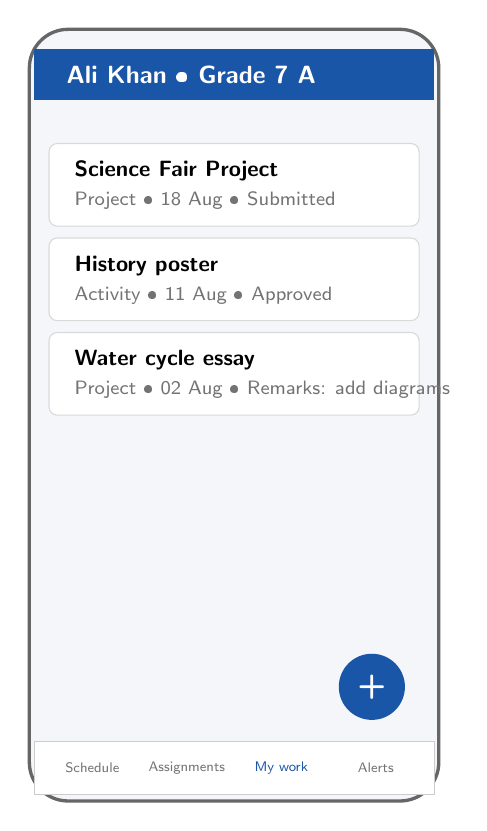
\begin{tikzpicture}[font=\sffamily]
  \phoneframe{Ali Khan \textbullet{}  Grade 7 A}
  \appcard{7.3}{}{Science Fair Project}{Project \textbullet{}  18 Aug \textbullet{}  Submitted}
  \appcard{6.1}{}{History poster}{Activity \textbullet{}  11 Aug \textbullet{}  Approved}
  \appcard{4.9}{}{Water cycle essay}{Project \textbullet{}  02 Aug \textbullet{}  Remarks: add diagrams}
  \fill[campusblue] (4.35,1.45) circle (0.42);
  \node[text=white] at (4.35,1.45) {\large\textbf{+}};
  \navbar
  \navitem{0.80}{Schedule}{black!55}
  \navitem{2.00}{Assignments}{black!55}
  \navitem{3.20}{My work}{campusblue}
  \navitem{4.40}{Alerts}{black!55}
\end{tikzpicture}
\caption{My work tab: upload with the + button and watch the review
status (illustration).}
\end{figure}

% ----------------------------------------------------------------------
\section{Alerts}

The same notification list as parents have -- students receive general
school announcements and messages meant for them.

\tipbox{Your attendance is recorded automatically by your ID card --
keep the card with you all day, and do not lend it to anyone.}

\chapter{Teacher Portal (web)}

Teachers open the CampusTrack website in any browser and sign in with
their teacher username. The portal shows five tabs:

\begin{center}
\textbf{Student progress} \textbullet{}  \textbf{Assignments \& notes} \textbullet{} 
\textbf{Parent feedback} \textbullet{}  \textbf{Student uploads} \textbullet{}  \textbf{Timetable}
\end{center}

All screenshots in this chapter are taken from the live system.

% ----------------------------------------------------------------------
\section{Student progress -- write a report about a student}

This is where you tell parents how their child is doing. Every report
you save is \textbf{instantly sent to the parent's phone}.

\begin{enumerate}[itemsep=2pt]
  \item Choose the \textbf{Section} (for example \emph{Grade 7 A}) --
        the \textbf{Student} list fills automatically.
  \item Choose the student and the \textbf{Date}.
  \item Choose a \textbf{Category}: Academic, Behaviour, Sports,
        HomeworkStatus, TestResult or Other.
  \item Type a short \textbf{Title} (e.g.\ ``Math quiz result''), an
        optional \textbf{Grade} (e.g.\ ``A'' or ``87\%'') and your
        \textbf{Remarks}.
  \item Click \textbf{Save \& notify parent}. Done -- the parent is
        notified immediately.
\end{enumerate}

\begin{figure}[H]
\centering
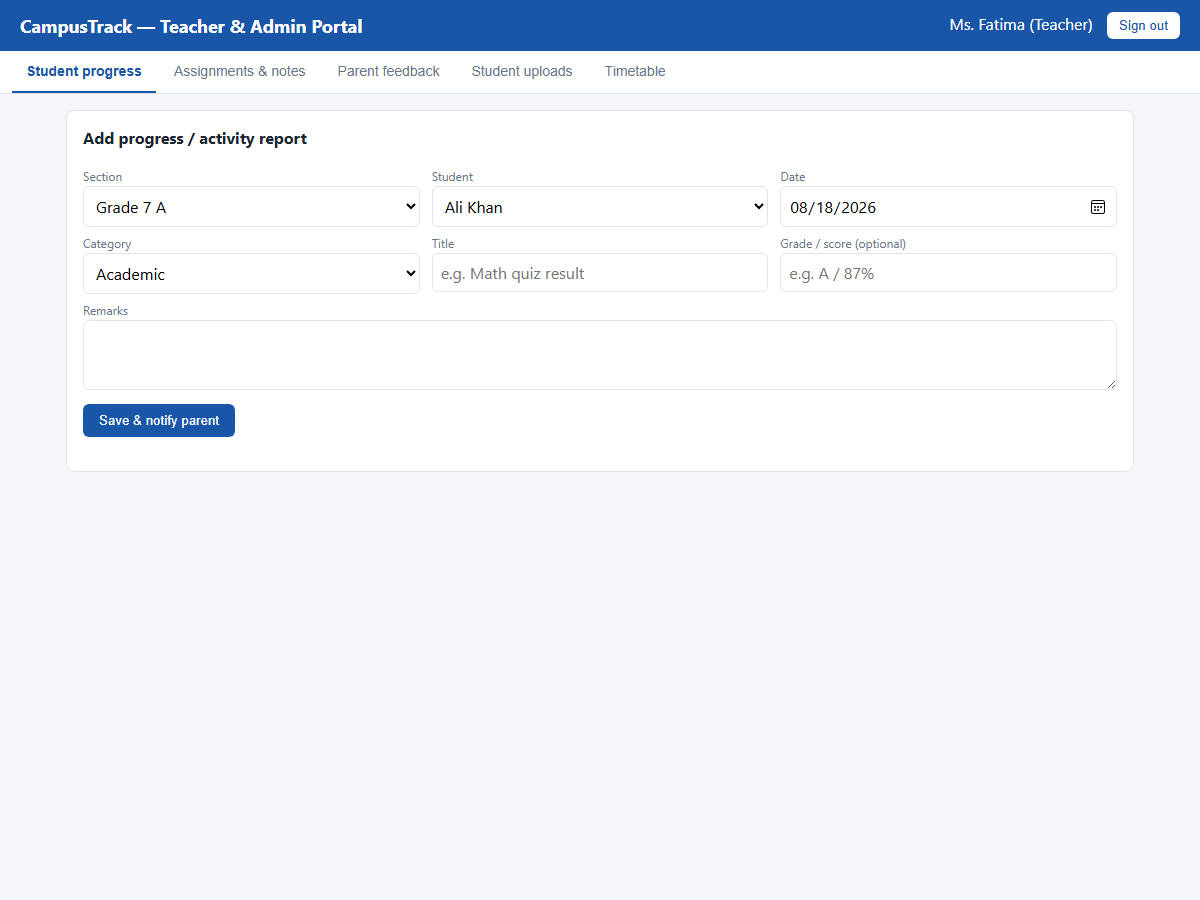
\includegraphics[width=\textwidth]{teacher-progress}
\caption{Student progress tab: pick section, student, category, and
write the report.}
\end{figure}

% ----------------------------------------------------------------------
\section{Assignments \& notes -- publish files with a QR code}

Upload an assignment or notes file once, and every student of the
section can download it -- from the list in their app, or by scanning
the QR code the portal gives you.

\begin{enumerate}[itemsep=2pt]
  \item Choose the \textbf{Section} and the \textbf{Type}
        (Assignment or Notes), and a \textbf{Due date} if relevant.
  \item Type the \textbf{Title} and a short \textbf{Description}.
  \item Click \textbf{Choose file}, pick your document, then click
        \textbf{Upload}.
  \item The portal immediately shows a \textbf{QR code}. Print it on
        the handout or project it on the class screen -- students scan
        it and receive the file instantly.
\end{enumerate}

\begin{figure}[H]
\centering
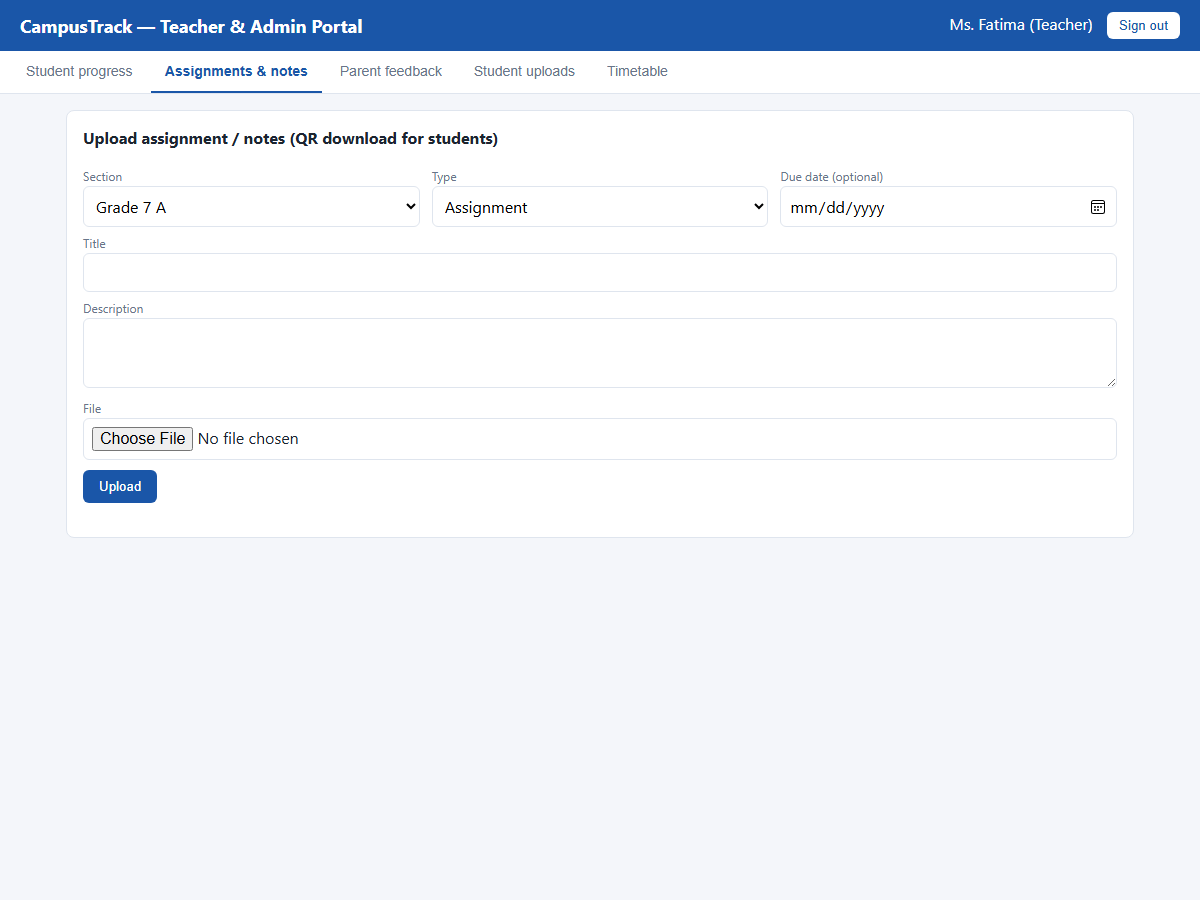
\includegraphics[width=\textwidth]{teacher-assignments}
\caption{Assignments \& notes tab: fill the form, upload the file, get
the QR code.}
\end{figure}

% ----------------------------------------------------------------------
\section{Parent feedback -- read and reply}

Every message a parent sends from the app lands in this inbox, with its
category, the parent's and student's names, and the current status.

\begin{enumerate}[itemsep=2pt]
  \item Read the message in the table.
  \item Click \textbf{Reply\ldots}, type your answer, press OK.
  \item The parent receives your reply as a phone notification, and the
        status changes to \emph{Replied}.
\end{enumerate}

\begin{figure}[H]
\centering
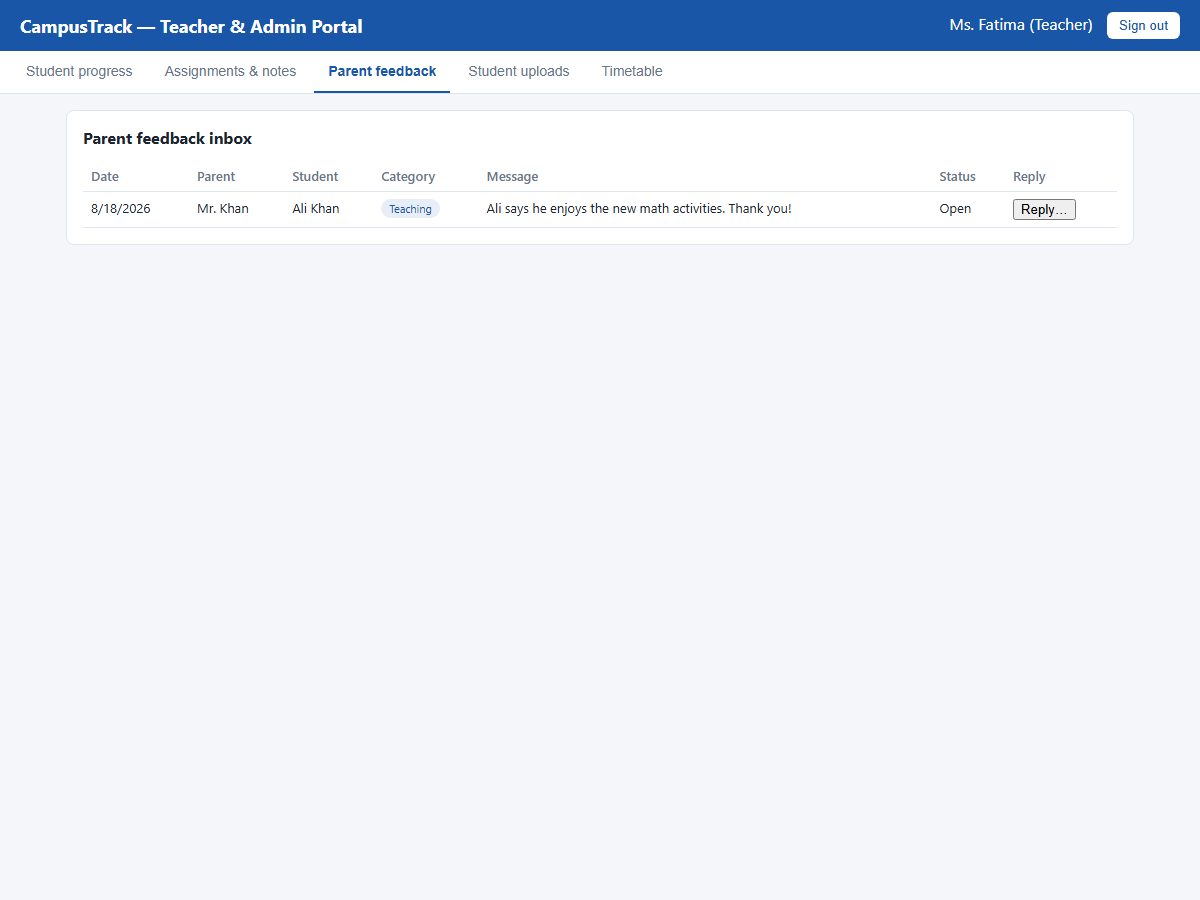
\includegraphics[width=\textwidth]{teacher-feedback}
\caption{Parent feedback inbox with a message from Mr.\ Khan in the
Teaching category.}
\end{figure}

% ----------------------------------------------------------------------
\section{Student uploads -- review submitted work}

When students upload projects, activities or theses from their app,
they appear here until reviewed.

\begin{enumerate}[itemsep=2pt]
  \item Click the file name to open and read the work.
  \item Click \textbf{Approve} or \textbf{Reject}.
  \item Optionally type remarks -- the student sees them under the
        upload in their app.
\end{enumerate}

\begin{figure}[H]
\centering
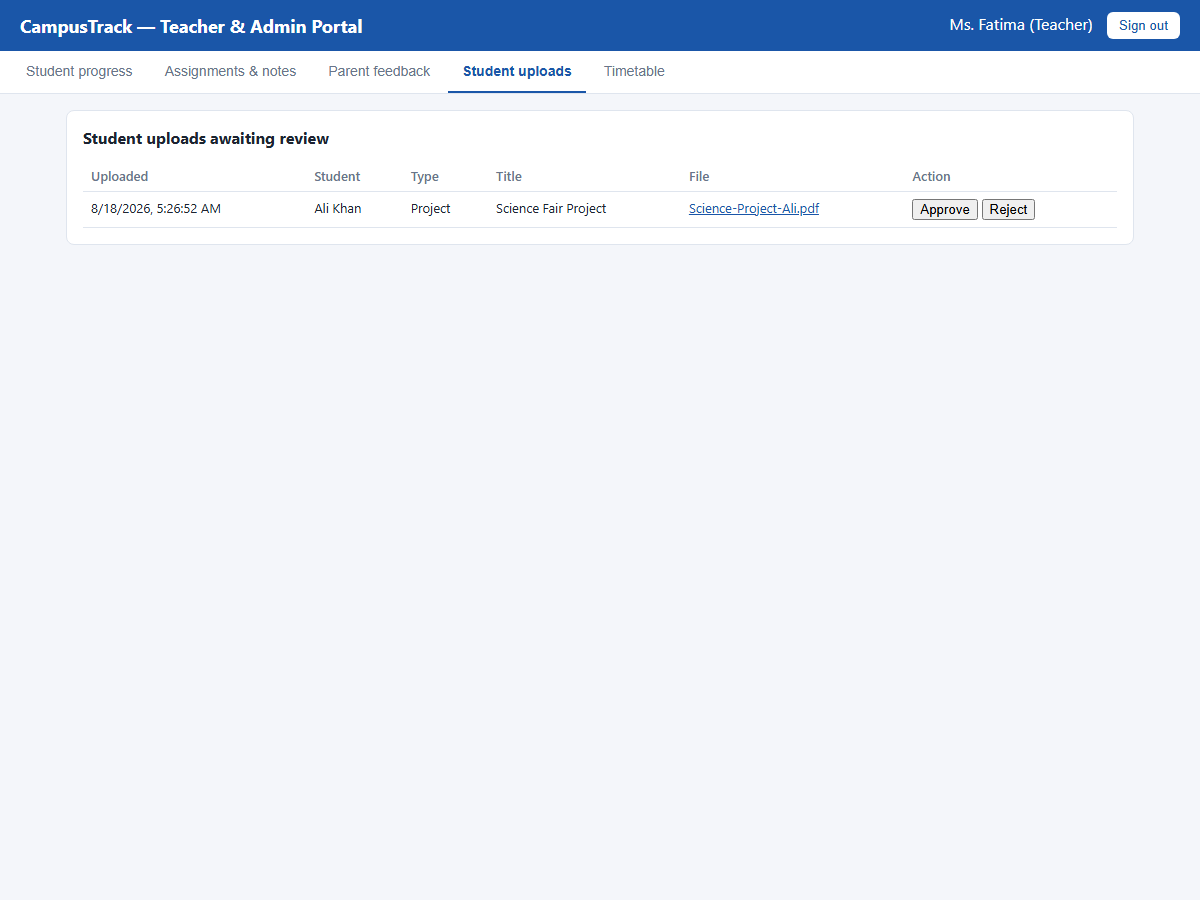
\includegraphics[width=\textwidth]{teacher-uploads}
\caption{Student uploads awaiting review -- here Ali Khan's Science
Fair Project.}
\end{figure}

% ----------------------------------------------------------------------
\section{Timetable -- view and add entries}

Teachers can view any section's full timetable and add entries for
their own subjects (day, start and end time, subject, teacher, room).
The timetable students and parents see in their apps updates instantly.

\begin{figure}[H]
\centering
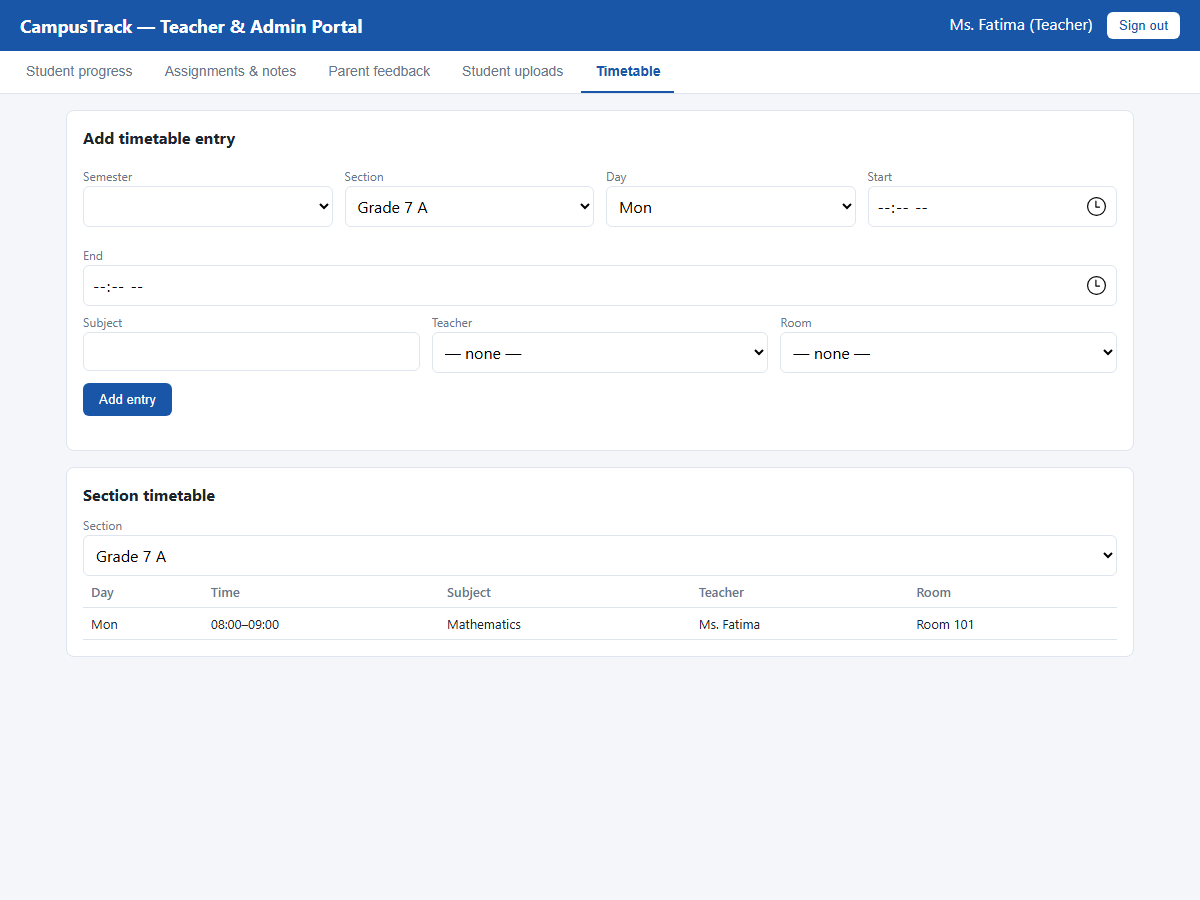
\includegraphics[width=\textwidth]{teacher-timetable}
\caption{Timetable tab: the entry form on top, the section's current
timetable below.}
\end{figure}

\tipbox{Everything a teacher saves -- reports, replies, assignments --
reaches parents and students \emph{immediately}. There is no separate
``publish'' step.}

\chapter{Admin Portal (web)}

Administrators sign in to the same web portal as teachers, but see one
extra tab: \textbf{Administration}. An admin can do everything a teacher
can, plus manage the school's structure and accounts.

% ----------------------------------------------------------------------
\section{Classes \& sections (fully modular)}

The school's structure is never fixed. At any time you can:

\begin{itemize}[itemsep=2pt]
  \item \textbf{Add a class}: type the name (``Grade 8'', ``BSCS-1'')
        and click \textbf{Add class}.
  \item \textbf{Add a section}: choose the class, type the section name
        (``A'', ``B'', ``Blue'') and click \textbf{Add section}.
  \item \textbf{Delete a class or section}: click \textbf{delete} next
        to it. Deletion is ``soft'' -- old attendance and reports are
        kept for the record, the class simply disappears from all
        lists.
\end{itemize}

% ----------------------------------------------------------------------
\section{Rooms \& RFID readers}

Register every physical location and the reader hardware on its door:

\begin{enumerate}[itemsep=2pt]
  \item \textbf{Add the room}: name it and pick its type -- Gate,
        Classroom, Laboratory, Library, DiscussionRoom, Auditorium or
        Other.
  \item \textbf{Add its reader}: type the reader code printed on the
        device (e.g.\ \texttt{GATE-01}), pick the room, and choose the
        number of antennas: \textbf{3 for gates, 2 for rooms}.
\end{enumerate}

From that moment the system understands the door: antenna order
$1\rightarrow2(\rightarrow3)$ means entry, the reverse means exit.

\begin{figure}[H]
\centering
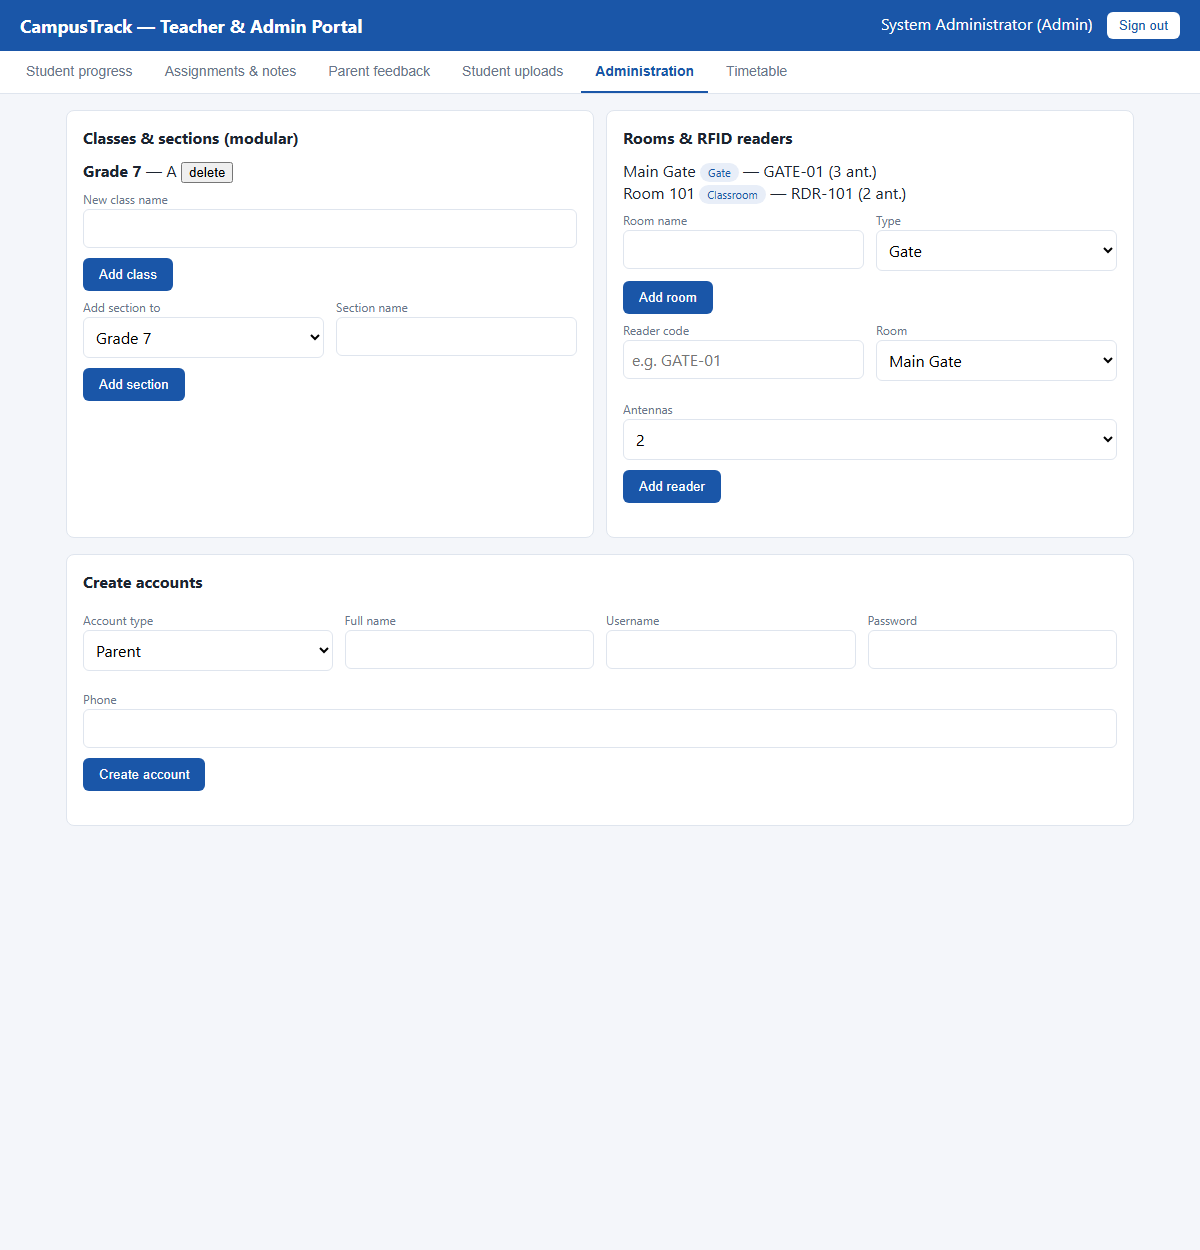
\includegraphics[width=\textwidth]{admin-structure}
\caption{The Administration tab: classes \& sections on the left, rooms
\& RFID readers on the right, account creation below.}
\end{figure}

% ----------------------------------------------------------------------
\section{Creating accounts}

Nobody registers themselves -- the admin creates every account. In
\textbf{Create accounts}:

\subsection{Create a parent}
Choose account type \textbf{Parent}, fill full name, username, password
and phone, click \textbf{Create account}. Hand the username and password
to the parent.

\subsection{Create a teacher}
Same steps with account type \textbf{Teacher}.

\subsection{Create a student (and link everything together)}
Choose account type \textbf{Student}. Extra fields appear:

\begin{itemize}[itemsep=2pt]
  \item \textbf{Reg.\ no} -- the student's registration number;
  \item \textbf{RFID tag EPC} -- the code of the RFID chip inside the
        student's ID card (your card printer or a handheld reader shows
        this code). This is what makes automatic attendance work;
  \item \textbf{Section} -- which class and section the student joins;
  \item \textbf{Parent} -- pick the parent account created earlier.
        This link is what routes gate alerts and summaries to the right
        parent's phone.
\end{itemize}

\notebox{If a student's ID card is lost, issue a new card and simply
update the RFID tag EPC on the student -- history stays intact.}

% ----------------------------------------------------------------------
\section{Semesters and the timetable}

Create a semester (name, start and end date, ``current'' flag), then
build each section's timetable in the \textbf{Timetable} tab: day,
start/end time, subject, teacher, room -- entry by entry. Parents and
students see changes in their apps immediately.

\begin{figure}[H]
\centering
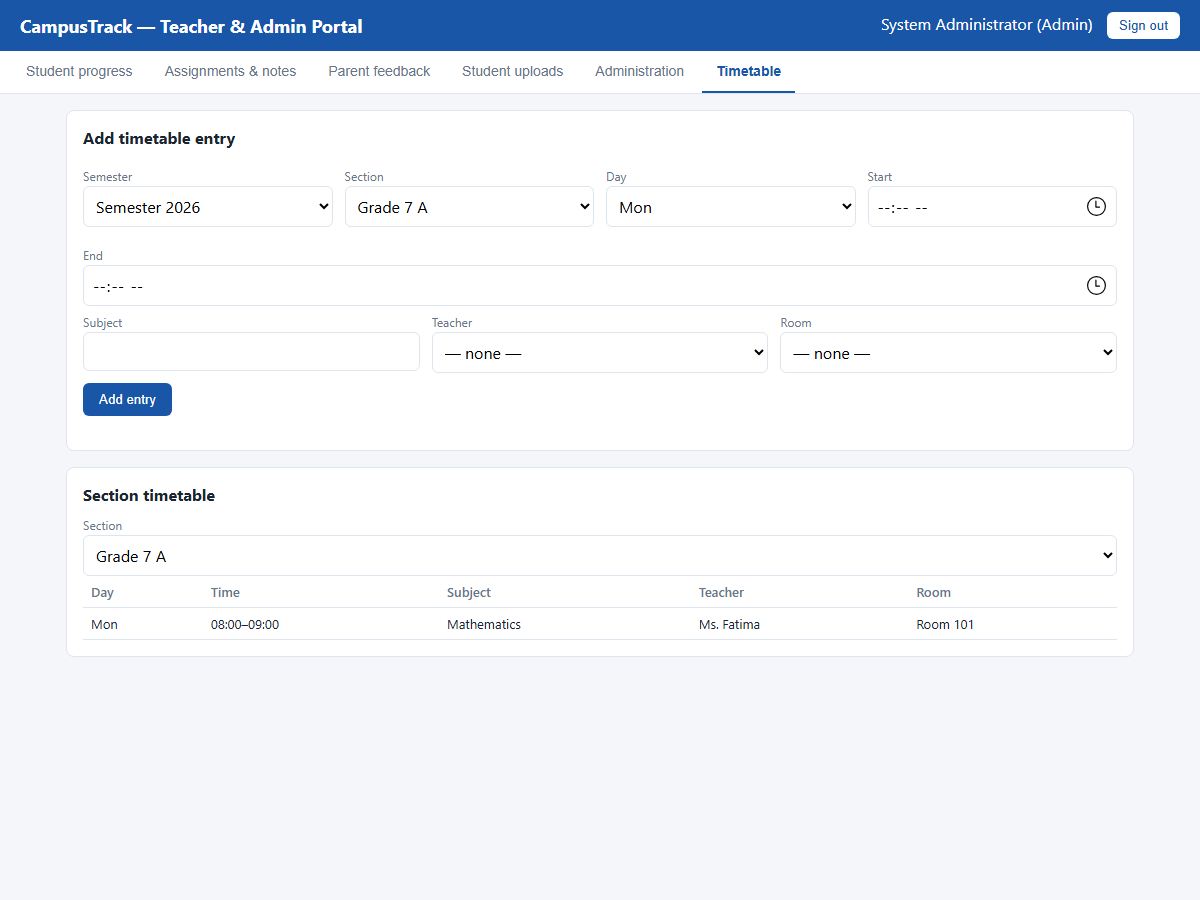
\includegraphics[width=\textwidth]{admin-timetable}
\caption{Building a section timetable as admin.}
\end{figure}

% ----------------------------------------------------------------------
\section{Daily \& weekly summary times}

By default parents receive the daily summary at \textbf{18:00} and the
weekly summary on \textbf{Friday}. Your IT person can change both in
the server settings (\texttt{Summaries:DailyTime},
\texttt{Summaries:WeeklyDay}).

% ----------------------------------------------------------------------
\section{Checklist: setting up a new school}

\begin{enumerate}[itemsep=2pt]
  \item Create the semester.
  \item Add classes and their sections.
  \item Add rooms, then the RFID reader of each room (3 antennas at
        gates, 2 elsewhere).
  \item Create teacher accounts.
  \item Create parent accounts.
  \item Create student accounts -- linking each student to a section, a
        parent, and the RFID EPC of their ID card.
  \item Build the timetable for every section.
  \item Ask parents and students to install the app and sign in.
\end{enumerate}

\tipbox{The default administrator login shipped with the system is
\texttt{admin} / \texttt{Admin@123} -- change this password on day
one.}

\chapter{Frequently asked questions}

\section*{For parents}

\textbf{I did not get a notification when my child reached school.}\\
Check that notifications are allowed for the CampusTrack app in your
phone settings, and that you have internet. The event is never lost --
open the app's \textbf{Attendance} tab to see it, and the daily summary
will include it.

\textbf{The app shows ``Absent'' but my child went to school.}\\
The child may have entered without the ID card, or the card may be
damaged. Ask the school office to test the card.

\textbf{I have two children in the school. Do I need two accounts?}\\
No. One parent account can be linked to any number of children -- use
the selector at the top of the app to switch.

\textbf{Can I choose in which language or at what time I get the daily
summary?}\\
The summary time is set by the school (usually 6:00 pm). Ask the school
office if a different time suits parents better.

\section*{For students}

\textbf{I scanned the QR code but nothing downloaded.}\\
Make sure you are connected to the internet and that the code is a
CampusTrack assignment code. Ask the teacher to re-print or re-project
the code if it is blurred.

\textbf{I uploaded the wrong file.}\\
Upload the correct file with the same title -- the teacher will see
both and review the newest one.

\textbf{Does the school see where I am all the time?}\\
No. The card is only noticed when you pass a door with antennas -- the
gate and room doors of the school. It records nothing anywhere else.

\section*{For teachers}

\textbf{Do parents really see my report immediately?}\\
Yes -- the moment you click \emph{Save \& notify parent}, a notification
goes to the parent's phone, and the report stays visible in their app.

\textbf{Which sections appear in my lists?}\\
The sections you teach according to the timetable. If a section is
missing, ask the admin to add your timetable entries.

\section*{For administrators}

\textbf{A reader stopped sending events.}\\
Check its power and network. All raw card reads are stored on the
server, so once the reader is back, attendance continues normally.

\textbf{Can we add a new building next year?}\\
Yes -- everything is modular. Add the new rooms and readers in the
Administration tab; no software change is needed.

\textbf{Is the students' data safe?}\\
Data lives in the school's own Microsoft SQL Server database. Every
user sees only what their role allows: parents only their own
children, students only themselves.


\end{document}
